\documentclass[letterpaper,12pt]{article}
\usepackage{float}
\usepackage{array}
\usepackage{threeparttable}
\usepackage{geometry}
\geometry{letterpaper,tmargin=1in,bmargin=1in,lmargin=1.25in,rmargin=1.25in}
\usepackage{fancyhdr,lastpage}
\pagestyle{fancy}
\lhead{}
\chead{}
\rhead{}
\lfoot{}
\cfoot{}
\rfoot{\footnotesize\textsl{Page \thepage\ of \pageref{LastPage}}}
\renewcommand\headrulewidth{0pt}
\renewcommand\footrulewidth{0pt}
\usepackage[format=hang,font=normalsize,labelfont=bf]{caption}
\usepackage{listings}
\lstset{frame=single,
  language=Python,
  showstringspaces=false,
  columns=flexible,
  basicstyle={\small\ttfamily},
  numbers=none,
  breaklines=true,
  breakatwhitespace=true
  tabsize=3
}
\usepackage{amsmath}
\usepackage{amssymb}
\usepackage{amsthm}
\usepackage{harvard}
\usepackage{setspace}
\usepackage{float,color}
\usepackage[pdftex]{graphicx}
\usepackage{hyperref}
\hypersetup{colorlinks,linkcolor=red,urlcolor=blue}
\theoremstyle{definition}
\newtheorem{theorem}{Theorem}
\newtheorem{acknowledgement}[theorem]{Acknowledgement}
\newtheorem{algorithm}[theorem]{Algorithm}
\newtheorem{axiom}[theorem]{Axiom}
\newtheorem{case}[theorem]{Case}
\newtheorem{claim}[theorem]{Claim}
\newtheorem{conclusion}[theorem]{Conclusion}
\newtheorem{condition}[theorem]{Condition}
\newtheorem{conjecture}[theorem]{Conjecture}
\newtheorem{corollary}[theorem]{Corollary}
\newtheorem{criterion}[theorem]{Criterion}
\newtheorem{definition}[theorem]{Definition}
\newtheorem{derivation}{Derivation} % Number derivations on their own
\newtheorem{example}[theorem]{Example}
\newtheorem{exercise}[theorem]{Exercise}
\newtheorem{lemma}[theorem]{Lemma}
\newtheorem{notation}[theorem]{Notation}
\newtheorem{problem}[theorem]{Problem}
\newtheorem{proposition}{Proposition} % Number propositions on their own
\newtheorem{remark}[theorem]{Remark}
\newtheorem{solution}[theorem]{Solution}
\newtheorem{summary}[theorem]{Summary}
%\numberwithin{equation}{section}
\bibliographystyle{aer}
\newcommand\ve{\varepsilon}
\newcommand\boldline{\arrayrulewidth{1pt}\hline}


\begin{document}

\begin{flushleft}
  \textbf{\large{Problem Set \#3}} \\
  MACS 30100, Dr. Evans \\
  Alice Mee Seon Chung
\end{flushleft}

\vspace{5mm}

\noindent\textbf{Problem 1: Some income data, lognirmal distrubution, and GMM}
 
 \textbf \\ {(a)} 
 
\begin{figure}[H]\centering\captionsetup{width=5.0in}
  \caption{\textbf{Histogram }}\label{Fig_1}
  \fbox{\resizebox{5.5in}{4.0in}{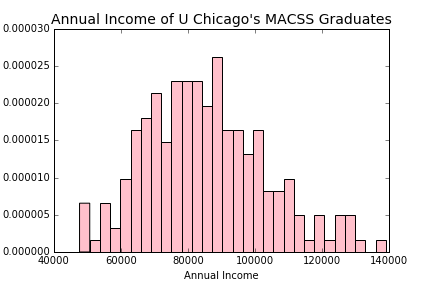
\includegraphics{Fig_1a.png}}}
 \end{figure}
  \newpage
  
 \textbf \\ {(b)} 
 
\begin{figure}[H]\centering\captionsetup{width=5.0in}
  \caption{\textbf{Plots}}\label{Fig_1}
  \fbox{\resizebox{5.0in}{4.0in}{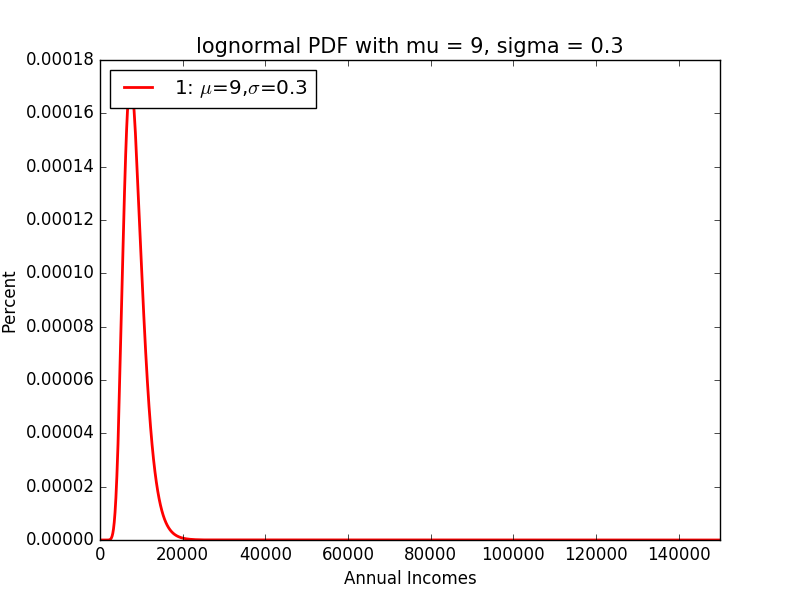
\includegraphics{Fig_1b.png}}}
 \end{figure}
 
\noindent\\
$\mu$ for GMM is 11.331880879623894 and $\sigma$ for GMM is 0.20869665796849818. The value of GMM criterion function at the estimated parameter values is 1.527969312041055e-15.\\
Data moments at the estimated parameter values; $\mu$ is 85276.82360625811 and $\sigma$ is 17992.542128046523.Model moments at the estimated parameter values; $\mu$Mu is 85276.82659818021 and $\sigma$ is 17992.542438137243.\\
Data moments and model moments are very close. We can say that GMM estimates well.
 
 \newpage
 
\textbf \\ {(c)} 
 
\begin{figure}[H]\centering\captionsetup{width=5.0in}
  \caption{\textbf{Plots}}\label{Fig_1}
  \fbox{\resizebox{5.0in}{4.0in}{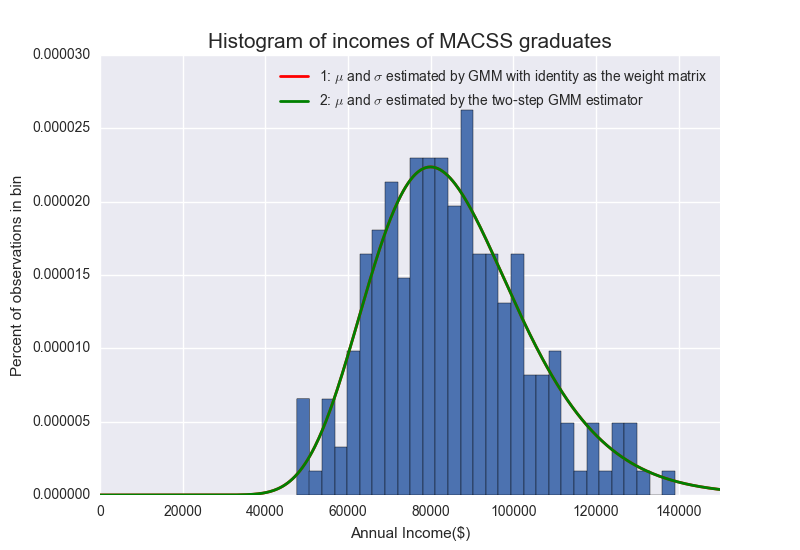
\includegraphics{Fig_1c.png}}}
 \end{figure}

\noindent\\ 
$\mu$ with the two-step GMM extimator is 11.331880875653171 and $\sigma$ with the two-step GMM extimator is 0.20869664411157565. The value of GMM criterion function at the estimated parameter values is 2.1285610191427995e-05.
Data moments at the estimated parameter values; $\mu$ is 85276.82360625811 and $\sigma$ is 17992.542128046523. Model moments at the estimated parameter values; $\mu$ is 85276.826012958121 and $\sigma$ is 17992.541093797605.\\
There are very small differences between data moments and model moments with two-step GMM. We can say that they are very close.
\\
\newpage

\textbf \\ {(d)} 
\begin{figure}[H]\centering\captionsetup{width=5.0in}
  \caption{\textbf{Plots}}\label{Fig_1}
  \fbox{\resizebox{5.0in}{4.0in}{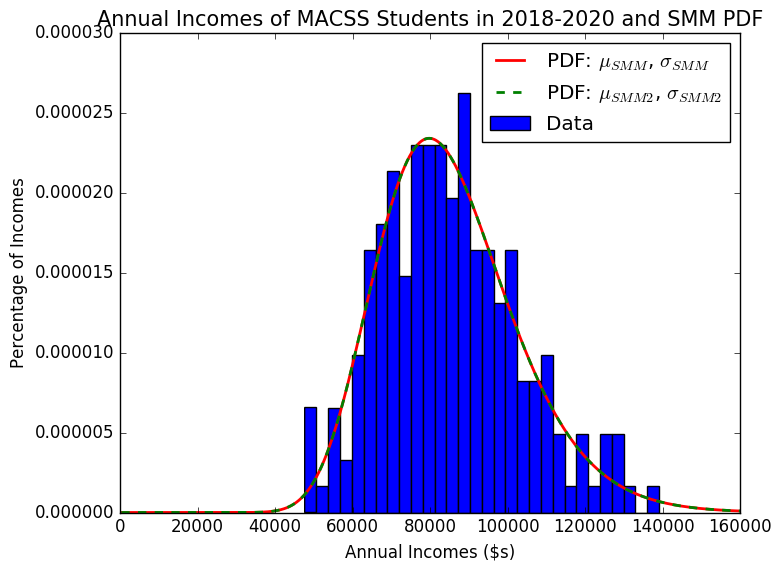
\includegraphics{Fig_1d.png}}}
 \end{figure}
\noindent\\  
Estimated $\mu$ with GMM using three moments is 11.335681500134852.
Estimated $\sigma$ with GMM using three moments is 0.21059989859759912.\\
The value of GMM criterion function at the estimated parameter values is\\ 1.218716526687726e-11.\\
Data moments at the estimated parameter values are: 0.3, 0.5, 0.2.\\
Model moments at the estimated parameter values are: 0.30000096942041676,\\ 0.4999971939215148, 0.20000183665806764.\\
Though we can see there are little differences between three data moments against three model moments, we can say that three model moments are very close to three data moments.

 \newpage
 
 \textbf \\ {(e)} 
 \begin{figure}[H]\centering\captionsetup{width=5.0in}
  \caption{\textbf{Plots}}\label{Fig_1}
  \fbox{\resizebox{5.0in}{4.0in}{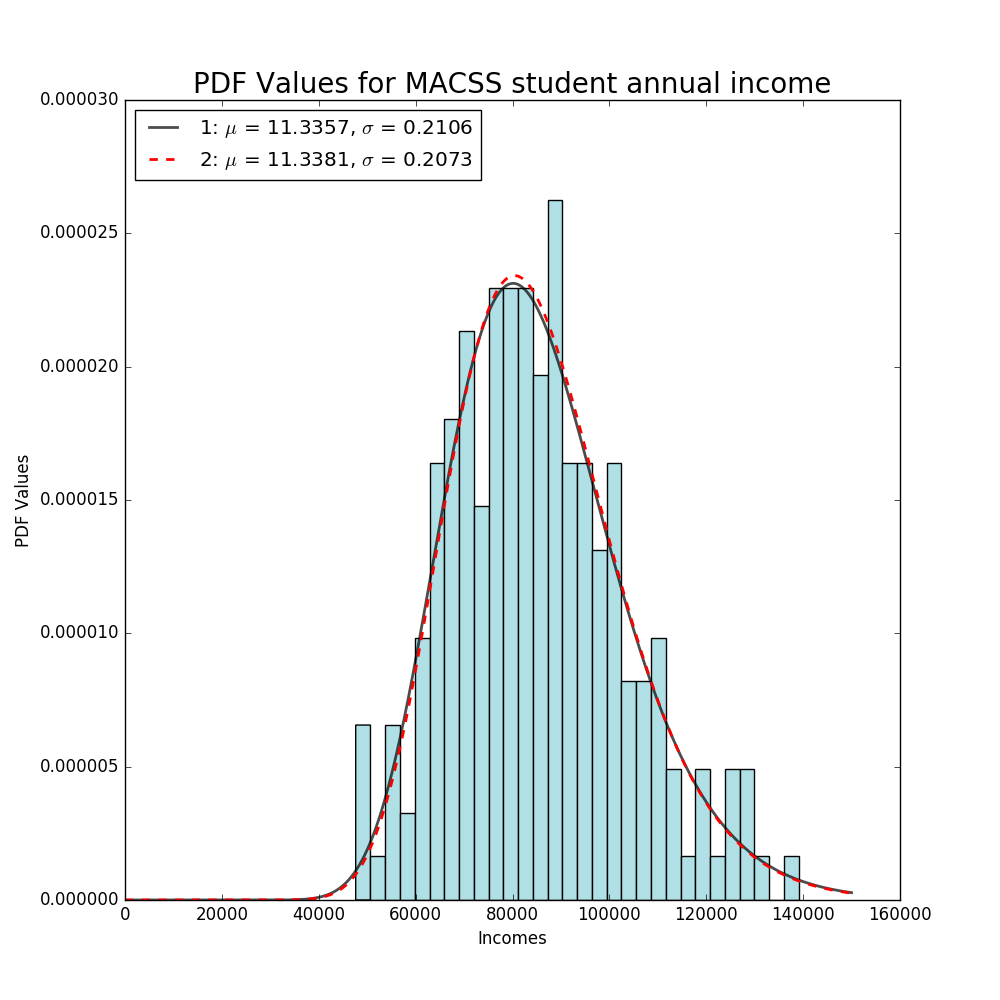
\includegraphics{Fig_1e.png}}}
 \end{figure}
 
\noindent\\
Estimated $\mu$ with two step GMM using three moments is 11.335682571476385. Estimated $\sigma$ with two step GMM using three moments is 0.21059846880532573.\\
The value of GMM criterion function at the estimated parameter values is 0.0005950032498406449.
Data moments at the estimated parameter values are 0.3, 0.5, 0.2.
Model moments at the estimated parameter values are 0.29999796279868857, 0.5000003760103441, 0.2000016611909666.\\
We can observe that there are very little differences between three data moments against three model moments with two setp GMM. However, we can say that three model moments are very close to three data moments.
\\
 \textbf \\ {(f)}\\
 \\
 Estimation from (e) fits the data best. All four estimations from (b),(c),(d),(e) fit well with the given data and actually they are in very close estimations. In figure3, (b) and (c) are very close in the plot and also in figure5, (d) and (e) are also very close in the plot. It is hard to tell the best estimation when you only consider graphs, so we have to consider all possible values derived from the data. With comparing the differences between data moments and model moments, (c) and (e) both perform better than (b) and (d). Then when we consider the plots, (e) covers slightly more in right tail and the data seems to be distributed more at the right tail according to the histogram. Thus I can conclude (e) fits the data best.\\
 \\
 
\noindent \textbf{Problem 2: Linear regression and GMM}
 \textbf \\  
 \\ {(a)} The GMM for $\beta_{0}$ is  0.2516447359381598, the GMM for $\beta_{1}$ is 0.01293345092463209, the GMM for $\beta_{2}$ is  0.4005011753872412, the GMM for $\beta_{3}$ is -0.009991695557197486.\\
The Value of criterion function is 0.00182128981702.



\end{document}
